\begin{center}
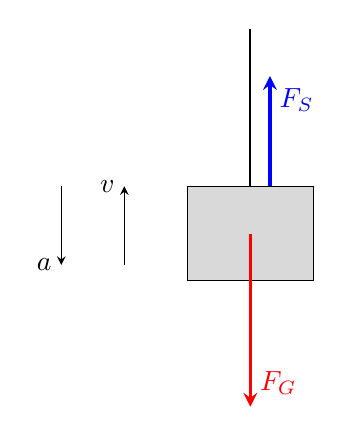
\begin{tikzpicture}[>=stealth]
 \draw[thick] (0,3.2) -- (0,1.2);
 \draw[fill=gray!30] (-0.8,0) rectangle (0.8,1.2);
 \draw[->, very thick, blue] (0.25,1.2) -- (0.25,2.6);
 \node[blue, right] at (0.25,2.3) {$F_\text{S}$};
 \draw[->, very thick, red] (0,0.6) -- (0,-1.6);
 \node[red, right] at (0,-1.3) {$F_\text{G}$};
 \draw[->] (-1.6,0.2) -- (-1.6,1.2) node[left] {$v$};
 \draw[->] (-2.4,1.2) -- (-2.4,0.2) node[left] {$a$};
\end{tikzpicture}
\end{center}

Die Last bewegt sich nach oben und wird abgebremst, die Beschleunigung zeigt also nach unten. Mit der Richtung nach oben positiv gilt für die Last
\begin{align}
 -m\,a &= F_\text{S} - m\,g
\end{align}
Die Seilkraft ist damit kleiner als die Gewichtskraft:
\begin{align}
 F_\text{S} &= \FKrF \\
   &= \mKr\cdot\left(\gE-\aKr\right) \\
   &= \FKr \approx \result{\FKrP{3}{2}}
\end{align}
